% Chapter Template

\chapter{Sample} % Main chapter title
\graphicspath{{Pictures/Chapter2}}
\label{Chapter 2} % Change X to a consecutive number; for referencing this chapter elsewhere, use \ref{ChapterX}

\lhead{Chapter 2. \emph{Sample}} % Change X to a consecutive number; this is for the header on each page - perhaps a shortened title

%----------------------------------------------------------------------------------------
%	SECTION 1
%---------------------------------------------------------------------------------------
\section{Introduction}



Give a brief of the chapter and introduce what you will talk about. 


\paragraph{Literature Survey}

This is a sample. Write about referred papers. Cite like this \citep{nip2010cyclic}. Another example would be this \citep{nip2010extremely}. More citations like this \citep{bird2004evaluating}, \citep {tremblay2003seismic} and \citep {alhamaydeh2016key}.

\paragraph{Research gaps}
Typically include research gaps for your study. 
\paragraph{Objective}
Similarly objectives of study. 
\paragraph{Scope}
Define scope of study. 
\paragraph{An algorithm}
How you could refer to figures: This is an example. (Refer \ref{fig5}). You can add equations like this Eq. (\ref{eq1})
\begin{equation}
\label{eq1}
  SDR = sd(T) - \sum_{i}\frac{{T}_{i}}{|T|}\times sd({T}_{i})
\end{equation}

\begin{figure}[]
\centering
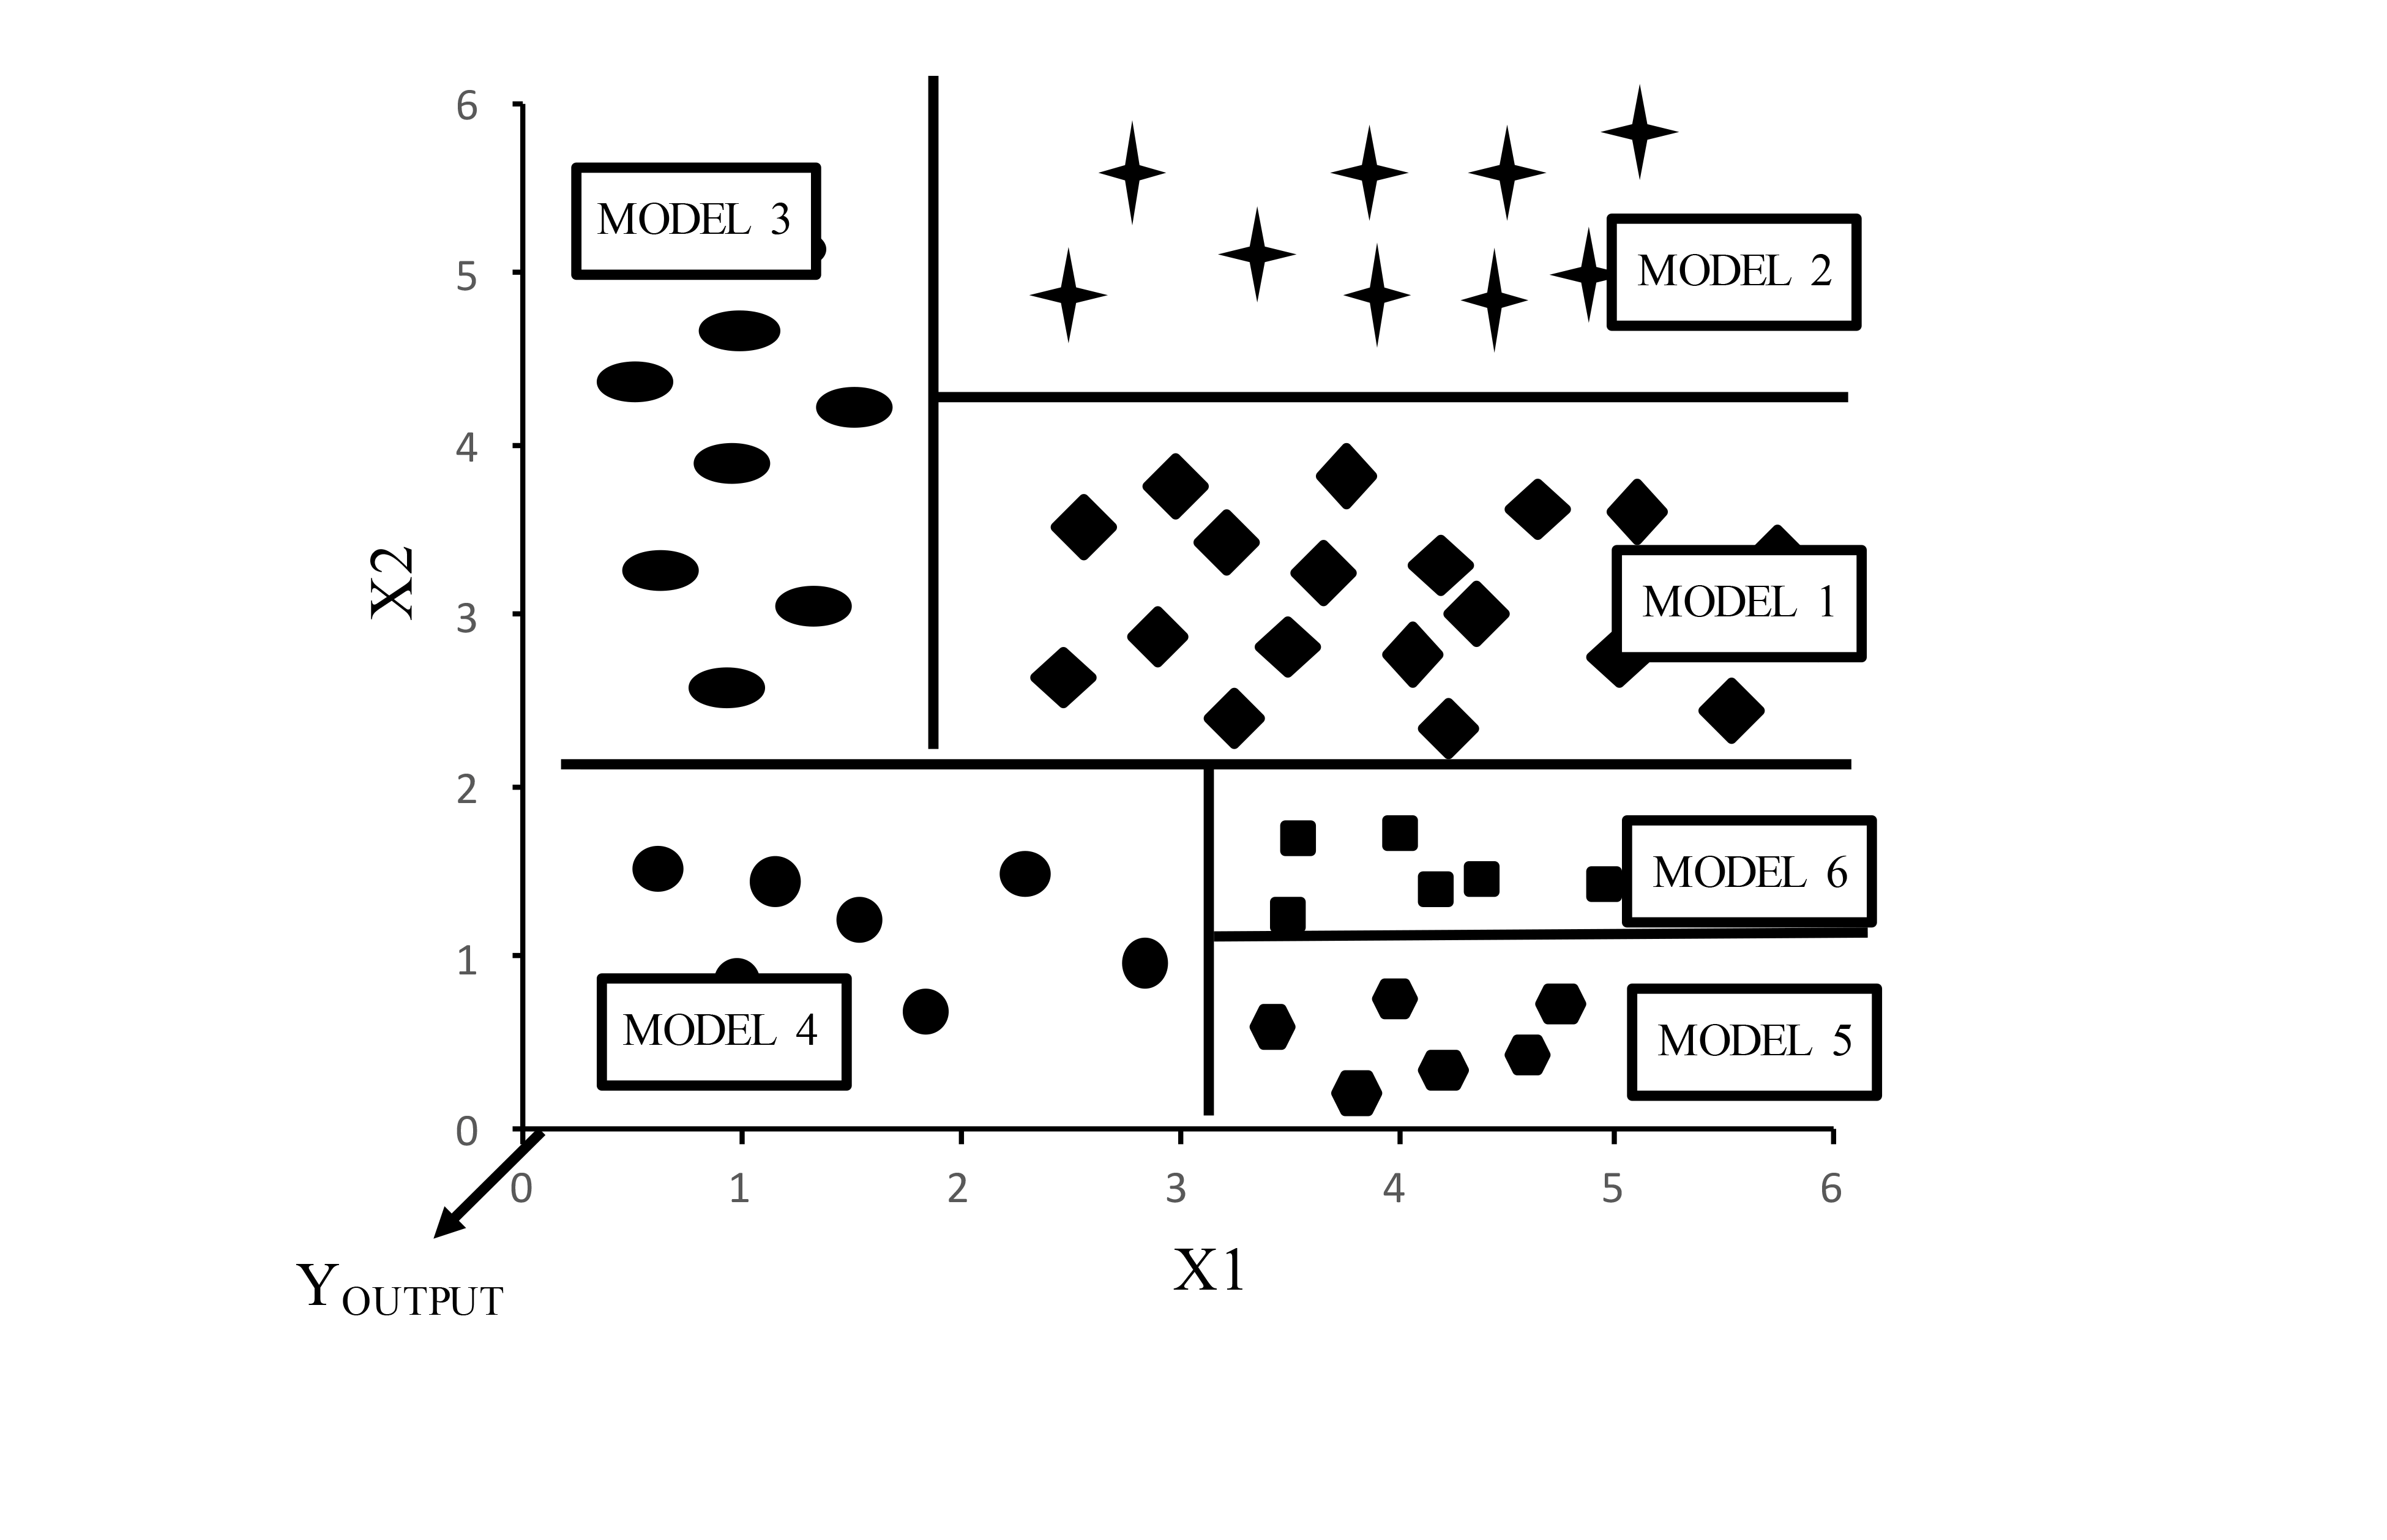
\includegraphics[height=7cm]{splits.png}
\caption{Splitting of the input space (X1 x X2) by M5' model tree algorithm}
\label{fig5}
\end{figure}

\section{Adding another section}
You can show a lot of figures together like these Figures \ref{fig61}, \ref{fig62}, \ref{fig63} below.
\begin{figure} [!htbp]
\centering    
\subfigure[Caption1]{\label{fig61}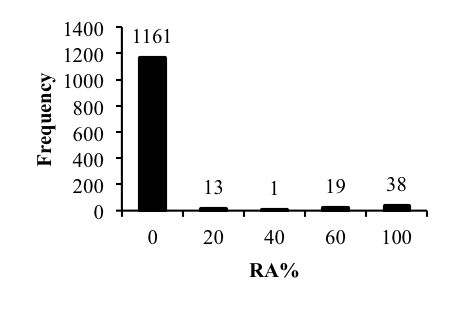
\includegraphics[width=42mm]{data1.png}}
\subfigure[Caption2]{\label{fig62}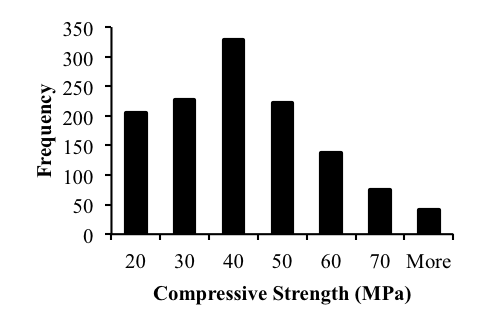
\includegraphics[width=42mm]{data2.png}}
\subfigure[Caption3]{\label{fig63}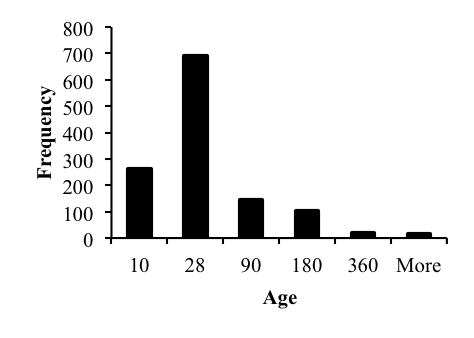
\includegraphics[width=42mm]{data3.png}}
\caption{Figures sample}
\end{figure}
You can add lists into the text like this. 
\begin{itemize}
\settowidth{\leftmargin}{{\Large$\square$}}\advance\leftmargin\labelsep
\itemsep3pt\relax
\renewcommand\labelitemi{{\lower1pt\hbox{\small$\square$}}}
\item	Some sample text item 1. 
\item You may refer to tables \ref{tab1} 
\item Or figures \ref{fig61}
\end{itemize}

Tables can be added like this
\begin{table}[!htbp]
\centering
\caption{Sample table}
\label{tab1}
\begin{tabular}{llll}

\hline
Column 1 & Column 2 & Column 3       \\\hline
1         & Data1 & 13.41179 & 0.9492839 \\
2            & Data2 & 13.39824 & 0.9492952\\\hline
\end{tabular}
\end{table}
